Achtung! In diesem Abschnitt werden viele Spielobjekte die bisher noch nicht genau beschrieben wurden gezeigt. Es kann für einen ersten Eindruck ganz sinnvoll sich die Benutzeroberfläche anzuschauen bevor Sie genau wissen wie die Details funktionieren. Um das Kapitel vollständig zu verstehen empfehlen wir allerdings nocheinmal an diese Stelle zurückzukehren, sobald Sie sich mit der Spiellogik auseinandergesetzt haben.
\section{Spieler-Interface}
% Aus dem Wiki
% ------------
%
% Siehe: https://sopra.informatik.uni-freiburg.de/soprawiki/index.php?title=GDD#Spieler-Interface
%
% Dieser Abschnitt beinhaltet eine Beschreibung des Spielbildschirms, also
% dessen, was für den Spieler sichtbar ist. Dies beinhaltet die Art der
% Darstellung (2D oder 3D), die Kamerasicht, usw.
%
% Wichtig ist, dass alle sichtbaren Elemente, wie Minimap, Menüleiste, etc.
% erklärt werden. Durch ein Bild eines typischen Vertreters dieser Spielart
% oder durch eine Konzeptzeichnung des Interfaces kann die Beschreibung noch
% verbessert werden. In der finalen Version des GDDs können auch Screenshots
% des eigenen Spiels verwendet werden.
%
% Außerdem wird in diesem Abschnitt erklärt, wie der Spieler das Spiel steuert
% (mit der Maus, mit Maus und Tastatur, Joystick, Gamepad usw.). Alle Aktionen,
% die der Spieler durchführen kann, müssen erklärt werden. Auch mögliche
% Shortcuts und/oder Tastenkombinationen sollten hier erwähnt werden.
%
%
% Aus den Folien
% --------------
%
% Siehe: https://sopra.informatik.uni-freiburg.de/soprawiki/images/1/11/How-To-GDD_SS19.pdf
%
% * Beschreibung dessen, was der Spieler sieht
% * Art der Darstellung, Kameraansichten, sichtbare Elemente (HUD, Minimap,
%   Menüleisten, usw.)
% * Bild (Konzeptzeichnung, Screenshot, Mockup) dessen, wie das Spiel aussehen
%   soll.
% * Beschreibung der Steuerung.
\begin{figure}[ht]
	\centering
	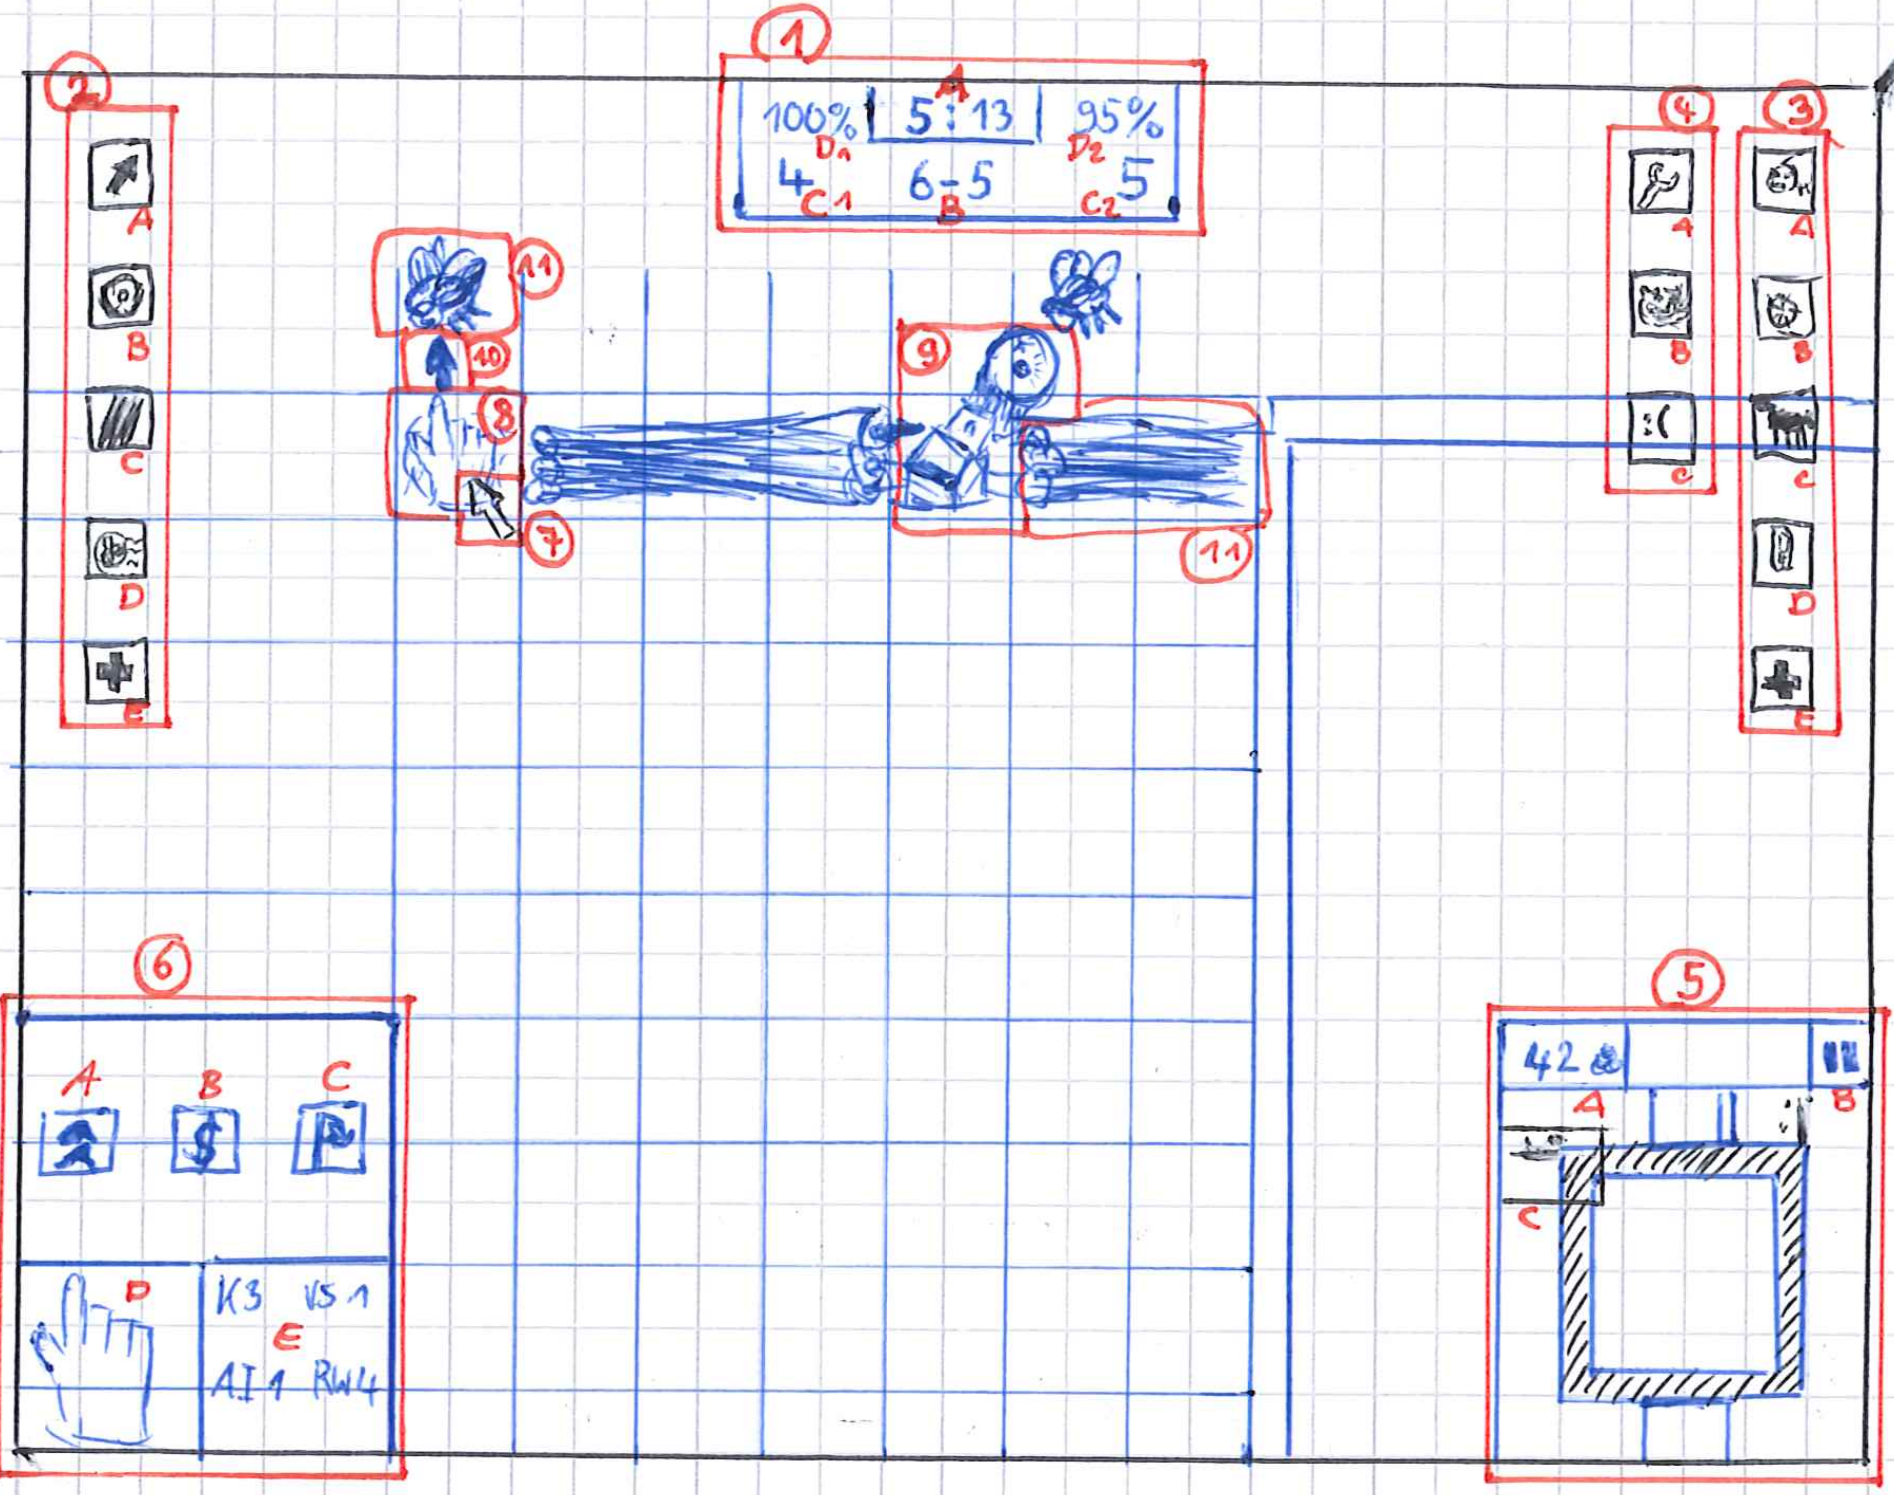
\includegraphics[width=1\textwidth]{spieler-interface.png}
	\caption{Spieler-Interface}
	\label{fig:spieler-interface}
\end{figure} \newpage
Abbildung \ref{fig:spieler-interface} zeigt eine typische Momentaufnahme des Spiels \textit{Kernel Panic!}.
Der Spieler betrachtet die Spielwelt aus der Top-Down Perpektive.\\
Beschreiben wir zunächst das Head-up-Display (HUD) bestehend aus den rot markierten Bereichen mit den Nummerierungen $1$ bis $7$:
\begin{itemize}
	\item{1 Spielstand} Hier werden die wichtigsten Informationen angezeigt um direkt einen Überblick ins Spiel zu bekommen, vergleichbar mit einem Punktestand.
	\begin{itemize}
		\item{$1 A$: Die aktuelle \textit{Spielzeit} zeigt an wieviele Minuten und Sekunden das aktuelle Spiel bereits im Gange ist.}
		\item{$1 B$: Direkt unter der \textit{Spielzeit} ist die Anzahl der erfolgreich besiegten \textit{Wellen} im Überblick zu sehen: links die eigenen, rechts die des Gegners.}
		\item{$1 C_{1}$ \& $1C_{2}$:} $C_{1}$ zeigt die \textit{Erfahrungspunkte}, die man sich erspielt hat, $C_{2}$ die des Gegners.
		\item{$D_{1}$ \& $D_{2}$:} Die aktuelle Ladung der Spieler. Hier gilt ebenfalls, links die eigenen auf der rechten Seite die des Gegners.
	\end{itemize}
	\item {$2$ Verteidigungsgebäude:} Oben, am linken Bildrand ist eine Liste an \textit{Verteidigungsgebäuden}. Um die verschiedenen Gebäude auszuwählen kann man die Tafeln $2 A$ bis $2 E$ benutzen.
	\item {$3$ \& $4$ Angriffseinheiten:} Auf der gegenüberliegenden Seite des Bildschirms befinden sich die \textit{Angriffseinheiten}. Dabei ist $3$ die Liste der \textit{Truppen} und $4$ die Liste der \textit{Helden}. Auch hier kann man mit den verschiedenen Tafeln ($3 A$ bis $3 E$ bzw $4 A$ bis $4 C$) die genaue Auswahl treffen.
	\item {$5$ Übersicht:}
	\begin{itemize}
		\item{$5 B$ Pause: Mithilfe von diesem Feld kann man das Spiel pausieren und auf die Menüstruktur (\ref{fig:menu}) zugreifen.}
		\item{$5 A$: Im unteren rechten Eck kann man eine Mini-map, wie man sie aus MOBAs oder Strategiespielen kennt sehen. Sie zeigt die gesamte Spielwelt abstrahiert.}
		\item{$5 C$: der aktuelle Kameraausschnitt ist auf der Mini-map markiert; man kann den Bildausschnitt symbolisch erkennen.}
	\end{itemize}
	\item {$6$ Auswahl-Tafel: Zeigt Informationen über ein aktuell ausgewähltes Spielobjekt.}	\begin{itemize}
		\item{$6 A$ bis $6 C$: Der hier ausgewählte Mauszeigerschütze hat drei mögliche Aktionen: \textbf{Verbessern ($6 A$)}, \textbf{Verkaufen ($6 B$)} und \textbf{Strategie wählen ($6 C$)}.}
		\item{$6 D$: Eine Ansicht der aktuellen Auswahl im Bildformat.}
		\item{$6 E$: Der Status zeigt die wichtigsten Daten über das ausgewählte Spielobjekt, hier \textit{Kosten} (K), \textit{Verteidigungsstärke} (VS), \textit{Angriffsintervall }(AI) und \textit{Reichweite} (RW)}
	\end{itemize}
	\item {$7$ Der Mauszeiger mit dem der Spieler die Auswahl trifft.} 
\end{itemize}
Die anderen sichtbaren Objekte bilden die Spielwelt. Ein wichtiger Teil davon ist die Strecke die in Felder unterteilt ist. Eines dieser Felder belegt das Verteidigungsgebäude \textbf{Mauszeigerschütze (7)}, der in dieser Spielsituation gerade seinen Angriff durchführt und \textbf{Mauszeiger (10)} auf einen \textbf{Bug (12)} schießt.\\
Zwei weitere Verteidigungsgebäude sind ebenfalls zu sehen: einige \textbf{Kabel (11)} und der \textbf{CD-Werfer (9)} der gerade eine CD abfeuert.

\section{Kamera}
Wie bereits erwähnt handelt es sich bei der Kamera von \textit{Kernel Panic!} um eine \textit{Top-down Perspektive}, wie man es aus den typischen Tower Defense Spielen (z.B. Plants vs. Zombies) kennt.
Sie liefert eine strategische Übersicht auf die 2D Grafik und lässt sich mit der \textit{Maus steuern}.
Bewegt man den Mauszeiger an einen Bildschirmrand scrollt man in die entsprechende Richtung über die Spielwelt.

%\section{Tastaturzuweisung}
